\documentclass[a4paper,10.0pt,twoside]{npr}

\usepackage{multicol,graphicx,lastpage,footmisc,fancyhdr,paralist,
tabularx,array,booktabs,caption,multirow,upgreek,mathrsfs,gensymb,color}
\usepackage[fancyhdr,space,fntef,fontset=ubuntu]{ctex}
\usepackage{amssymb,bm,mathrsfs,bbm,amscd}
\usepackage{flushend,cuted}
\usepackage{refcount}
\usepackage{savesym}
\usepackage{textcomp}
\usepackage[tbtags]{amsmath}  %
\savesymbol{iint}
\usepackage{amstext} %数学宏包文本命令
\usepackage{balance} %版心底部对齐

\flushbottom      %版心底部对齐
\setcounter{section}{0}
\begin{document}
%\begin{CJK*}{GBK}{\song}{\wuhao}{\rm}

%___________________________________________________________________________________
\def\rd{{\rm d}}

\newcommand{\RM}{\ensuremath{\mathrm}}   %正体 既可用于文本模式也可用于数学模式
\newcommand{\dif}{\mathrm{d}}  %直立体d
\newcommand{\me}{\mathrm{e}}  %直立体e
\newcommand{\mi}{\mathrm{i}}  %直立体i
\newcommand{\mj}{\mathrm{j}}  %直立体j
\newcommand{\afrac}[2]{\dfrac{\,#1\,}{\,#2\,}}  %略长分数线
\newcommand{\nn}{\nonumber}  %公式无编号
\newcommand{\nt}{\noindent}
\newcommand{\OO}{~\text{。}}
\newcommand{\PP}{~\text{,}}
\newcommand{\OP}{~\text{;}}
\newcommand{\LT}{\left}
\newcommand{\RT}{\right}

%___________________________________________________________________________________

\balance
\fancypagestyle{myfoot}
{%
\fancyhf{}
\fancyhead[c]{\wuhao\song 高~等~核~物~理~实~验}
\renewcommand{\headrule}{\vskip 2pt
\hrule height0.4pt width\headwidth \vskip1pt
\hrule height0.4pt width\headwidth \vskip-1.8pt}
}%
\thispagestyle{myfoot}

%%%%%%%%%%%%%%%%%%%%%%%%%%%%%%%%%%%%%%%%%%%%%%%%%%%%%
%    奇偶页眉
%%%%%%%%%%%%%%%%%%%%%%%%%%%%%%%%%%%%%%%%%%%%%%%%%%%%%
\pagestyle{fancy}
\fancyhead{}
\fancyhead[ce]{\xiaowu\song \hspace{0.5em}高~等~核~物~理~实~验}
%\fancyhead[ro,le]{\xiaowuhao \hspace{0.5em}\textbf{\textperiodcentered}\;\thepage\;\textbf{\textperiodcentered}\hspace{0.5em}}
%\fancyhead[ce]{\xiaowu\song 粒~子~物~理~与~原~子~核~物~理~专~题~实~验}
%\fancyhead[re]{\xiaowu\song \hspace{0.5em}第\;31\;卷\hspace{0.5em}}
\fancyfoot[ce,co]{}
\renewcommand{\headrule}{\vskip 2pt
\hrule height0.4pt width\headwidth}


\setcounter{page}{001}%
\fancyhead[co]{\xiaowuhao\song  乔颢:康普顿散射}    %奇页页眉
\begin{center}
\title{%
\xiaoerhao \bf  %章标题为两行时改为 \exiaoer
康普顿散射\\[-5mm]}
\maketitle
\large \fs
乔颢$^{^1}$\\[2mm]

\xiaowu \song
1. 北京大学物理学院,海淀区 北京 100871;\\[4mm]

 
\footnotetext[0]{{\bf 作者简介:}~~\begin{minipage}[t][4.2mm]{149mm}\song
乔颢,E-mail: i@catofes.com
\end{minipage} }
%\footnotetext[0]{{\bf 通信作者:}\song ~~E-mail: xxx@xxx.xxx }%通信作者为第一作者时不要此项

\parbox{158mm} {
\zywu{\bf 摘要:}~~\fs
该实验使用NaI(Tl)闪烁提探测器测量了康普顿散射中散射光子能量和散射角之间的关系,验证了散射光子的能量随散射角增大而减小的结论。同时测量了不同散射角度下的相对散射截面,验证了散射截面也随散射角增大而减少。
\\
{\bf 关键词:}~~\fs 康普顿散射,微分散射截面,NaI(Tl)谱仪}\\
\end{center}
%%%%6.正文
\vspace{5mm}
%%%%6.正文
\setcounter{section}{0}
\begin{multicols}{2}
%----------------
%____________________________________________________________________________
%%%%以上请不要改动%%%%%%%%%%%%%%%%%%%%%%%%%%%%%%%%%%%%%%%%%%%%

\section{引言}    %1
\vspace*{-1mm}
\song\wuhao

康普顿散射是物质与射线相互作用的三种主要效应之一。 1923年康普顿的X射线散射实验从实验上证实了光子的粒子性,其具有能量$E=\hbar\omega$以及动量$\hbar k$。在微观光子和电子的相互作用中,康普顿散射实验证明了能量和动量守恒仍然成立。因为其在近代物理学史上的重要作用,1927年康普顿被授予诺贝尔物理学奖。

康普顿散射在各个方面都有着广泛的应用。因为高能X射线和生物体内物质之间最可能发生的作用就是康普顿散射,因而其是放射生物学的一个重要理论。同时利用康普顿散射还可以测量得到物质中的电子波函数。
\section{实验}
\subsection{实验介绍及原理}

康普顿散射是射线与物质相互作用的三种效应之一,具体指入射光子和原子核外电子产生碰撞而被散射的过程。入射光子将一部分能量传递给电子,使其脱离原子形成反冲电子。因为能量守恒的动量守恒,光子的频率和方向也会发生相应的变化。如图所示:

\begin{center}
   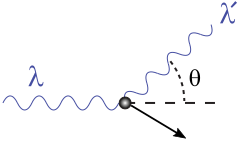
\includegraphics[width=0.4\textwidth]{CS.png}
\\
\xiaowu\song 图~1\begin{minipage}[t]{75mm} \quad 康普顿散射示意图。入射光子被散射角度为$\theta$。\\[-1mm]\wuhao
\end{minipage}
\end{center}

散射后光子的波长$\nu'$与入射光子波长$\nu$之间的关系如下:
\begin{equation}
   h\nu'=\frac{h\nu}{1+\frac{h\nu}{m_0c^2}(1-\cos{\theta})}
\end{equation}
其中$\theta$是光子的散射角。

本实验使用NaI(Tl)闪烁谱仪测量各个散射角度时散射光子的能谱,并有光电峰位和光电面积计算出散射光子能量,从而计算微分散射截面的相对值。

微分散射截面是指一个能量为$h\nu$的入射光子和一个核外电子作用后被散射到$\theta$方向上单位立体角的概率, 记作$\frac{d\sigma(\theta)}{d\Omega}$。由定义可以得到,当入射$N_0$个光子和$N_e$个电子相互作用后,探测器在$\theta$方向探测到的光子数目为
\begin{equation}
   N(\theta)=\frac{d\sigma(\theta)}{d\Omega}N_0N_e\Omega f
\end{equation}
其中$\Omega$为探测器对散射样品张角,f为散射样品自吸收因子,本实验中认为其为常数。

因为探测器效率的问题,探测器探测到的光子数目$N_p(\theta)$满足
\begin{equation}
   N_p(\theta)=N(\theta)R(\theta)\eta(\theta)\frac{4\pi}{\Omega}
\end{equation}
其中$\eta(\theta)$为探测器对点源总探测效率,$R(\theta)$为探测器峰总比。

由此可以得到微分散射截面的相对值即为:
\begin{equation}
    \frac{d\sigma(\theta)}{d\Omega}/\frac{d\sigma(\theta_0)}{d\Omega}=\frac{N_p(\theta)}{R(\theta)\eta(\theta)}/\frac{N_p(\theta_0)}{R(\theta_0)\eta(\theta_0)}
 \end{equation} 

\subsection{实验过程}

本实验中实验装置图如下:
\begin{center}
   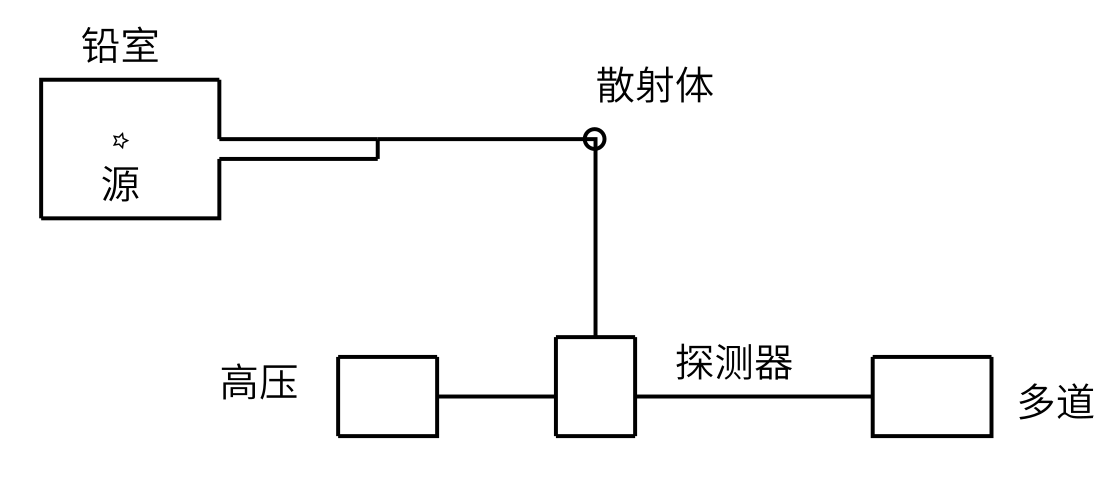
\includegraphics[width=0.45\textwidth]{shiyitu.png}
\\
\xiaowu\song 图~2\begin{minipage}[t]{75mm} \quad 实验装置示意图。\\[-1mm]\wuhao
\end{minipage}
\end{center}
源为$^{137}$Cs,它发射出0.662MeV的$\gamma$光子,经过准直后入射到样品,经样品散射到达位于30cm外的NaI(Tl)探测器。探测器可以旋转选择不同的散射角,并由此计算得到不同角度的相对微分散射截面。

具体的实验步骤如下:
\begin{enumerate}
\item 按照上图连接实验装置,不加入散射样品,直接使用探测器测量源的出射能谱。调整探测器的电压到合适值,并调整探测器的线性放大器使得Cs的光电峰落在460道左右。
\item 旋转探测器,测量不同角度散射能谱以及本地谱。
\item 利用$^{60}$Co源和Cs源对探测器进行标定。
\end{enumerate}

\section{实验结果和讨论}

 首先调整探测器的高压和放大。高压调整到580V,放大器放大倍数选择为30倍,此时Cs的0.644MeV峰落在464道处。

 测量得到不同角度的散射峰数据表如下:

 \begin{center}
\bgliu
{\bf 表~1\quad
不同角度散射峰数据表。每组数据的测量时间为10min。各栏具体说明见下文。}\\[0.5mm]
\renewcommand{\arraystretch}{1.5}
\liuhao\song\rm
\newcolumntype{M}{>{\centering\arraybackslash}m{10mm} >{\centering\arraybackslash}m{8mm}
>{\centering\arraybackslash}m{8mm}>{\centering\arraybackslash}m{8mm}>{\centering\arraybackslash}m{8mm}>{\centering\arraybackslash}m{8mm}>{\centering\arraybackslash}m{8mm}}
\begin{tabular}{M}
\specialrule{0.1em}{1pt}{1pt}

角度/度  &  峰位 &  峰高 &  左界 &  右界 &  计数 &  本底 \\
\midrule
20 &  427   &  728   &  393   &  457   &  37212 &  417   \\
40 &  361   &  545   &  325   &  389   &  24697 &  441   \\
60 &  286   &  473   &  253   &  309   &  18932 &  486   \\
80 &  225   &  514   &  200   &  249   &  17083 &  563   \\
100   &  184   &  632   &  163   &  202   &  17469 &  564   \\
120   &  155   &  819   &  139   &  172   &  19152 &  698   \\
\specialrule{0.1em}{3pt}{2pt}\\[-4mm]
\end{tabular}\\
\renewcommand{\arraystretch}{1.0}
\end{center}
表中角度极为光子的散射角,峰位为散射能谱中峰所在的道数,峰高为该道数的计数。由峰高可以给出重点区,重点区的左右边界的计数数为逢高的1/3左右。上表中的左右界即为重点区的边界。计数指重点区内所有的计数和。本底则指不放源时候重点区内的计数和。由此我们就可以得到不同角度下强度的相关信息。

通过Co源标定探测器能量,可以得到其1.17MeV和1.33MeV对应的道数分别为847道以及968道,结合Cs源的结果可以拟合出标定结果:
\begin{equation}
   E(MeV)= 0.00133x +0.047 
\end{equation}

根据标定结果我们可以计算得到不同角度散射光子实际的能量,如下表所示:

 \begin{center}
\bgliu
{\bf 表~2\quad
不同角度下散射光子能量和角度关系。}\\[0.5mm]
\renewcommand{\arraystretch}{1.5}
\liuhao\song\rm
\newcolumntype{M}{>{\centering\arraybackslash}m{20mm} >{\centering\arraybackslash}m{20mm}
>{\centering\arraybackslash}m{20mm}}
\begin{tabular}{M}
\specialrule{0.1em}{1pt}{1pt}

角度/度  &  能量/MeV   &  理论能量/MeV \\
\midrule
20 &  0.615 &  0.614 \\
40 &  0.527 &  0.508 \\
60 &  0.427 &  0.402 \\
80 &  0.346 &  0.320 \\
100   &  0.292 &  0.263 \\
120   &  0.253 &  0.225 \\
\specialrule{0.1em}{3pt}{2pt}\\[-4mm]
\end{tabular}\\
\renewcommand{\arraystretch}{1.0}
\end{center}

\begin{center}
   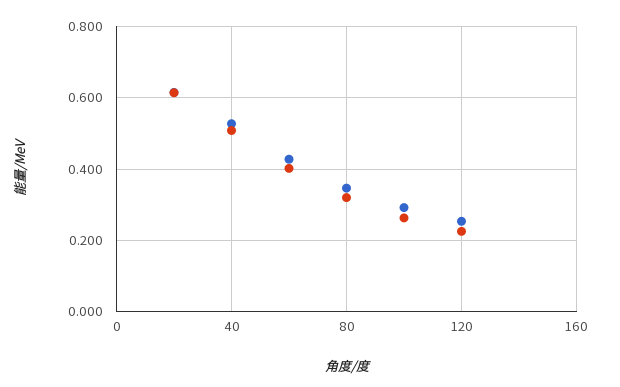
\includegraphics[width=0.45\textwidth]{nengliang.png}
\\
\xiaowu\song 图~3\begin{minipage}[t]{75mm} \quad 不同角度下散射光子能量\\[-1mm]\wuhao
\end{minipage}
\end{center}
从图中可以看出,散射能量随着散射角度的增大而减小。但是测量值和计算之间还是有着很大的差异的,在能量越小的时候差异越大。造成这个偏差的原因我不是特别的能解释,我猜测可能和以下的几个因素有关。首先在散射角较大的时候,实际观测的峰并不是特别的平滑,感觉10min的测量时间还是会带来一定的统计误差。还有我觉得很有可能在标定上出现了问题,因为理论能量和实际能量成一非常好的的线性关系,如下图所示。而标定的时候只有三个数据点,分辨是最先测量的Cs以及最后测量的Co的两个光电峰。如果标定和测量之间仪器状态稍微有了变化,那么很有可能不能明显的从标定数据中看到,所以很有可能是因为标定前后仪器状态有所改变而造成的偏移。

\begin{center}
   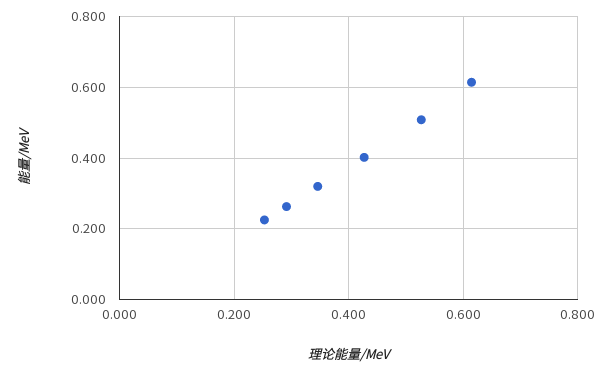
\includegraphics[width=0.45\textwidth]{cuowu.png}
\\
\xiaowu\song 图~4\begin{minipage}[t]{75mm} \quad 实测光子能量和理论光子能量关系图\\[-1mm]\wuhao
\end{minipage}
\end{center}

随后就可以计算不同角度下的相对散射截面了,数据如下表:

 \begin{center}
\bgliu
{\bf 表~3\quad
微分散射截面计算表。表中$R(\theta)$ 以及  $\eta(\theta)$是通过查表并利用二次样条曲线插值得到的结果。净面积为重点区总计数减去本底计数。}\\[0.5mm]
\renewcommand{\arraystretch}{1.5}
\liuhao\song\rm
\newcolumntype{M}{>{\centering\arraybackslash}m{10mm} >{\centering\arraybackslash}m{14mm}
>{\centering\arraybackslash}m{6mm}>{\centering\arraybackslash}m{10mm} >{\centering\arraybackslash}m{10mm}
>{\centering\arraybackslash}m{12mm}}
\begin{tabular}{M}
\specialrule{0.1em}{1pt}{1pt}

角度/度  &  能量/MeV   &  $R(\theta)$ &  $\eta(\theta)$ &  净面积   &  相对微分散射截面 \\
\midrule
20 &  0.615 &  0.418 &  0.000672 &  36795 &  1.000 \\
40 &  0.527 &  0.471 &  0.000756 &  24256 &  0.520 \\
60 &  0.427 &  0.557 &  0.000798 &  18446 &  0.317 \\
80 &  0.346 &  0.656 &  0.000859 &  16520 &  0.224 \\
100   &  0.292 &  0.735 &  0.000928 &  16905 &  0.189 \\
120   &  0.253 &  0.797 &  0.000981 &  18454 &  0.180 \\
\specialrule{0.1em}{3pt}{2pt}\\[-4mm]
\end{tabular}\\
\renewcommand{\arraystretch}{1.0}
\end{center}
将微分散射截面画出如下:
\begin{center}
   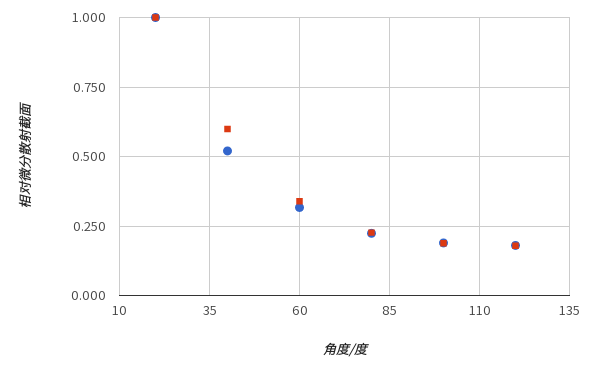
\includegraphics[width=0.45\textwidth]{ssjm.png}
\\
\xiaowu\song 图~5\begin{minipage}[t]{75mm} \quad 相对微分散射截面随散射角变化图。蓝线为测量值,红线为理论计算值。\\[-1mm]\wuhao
\end{minipage}
从图中可以看出相对微分散射截面随着散射角变大而逐渐变小。实际测量值和理论之有一定的误差。但是因为先前验证能量时就已经后很大的偏差了,所以这里实际偏差变小了的可信度并不高。相对微分散射截面的误差来源也有很多地方,在散射角较大能量较小的时候,因为探测器分辨率的原因,散射峰的峰位,峰高都不是特别的容易区分确定,因而造成重点区选择时候会带来很大的误差。同时重点区的选取方式也是一个经验性的方法,其本身可能会带来一定的误差。
\end{center}
\section{总结和结论}
本实验中使用了NaI(Tl)谱仪测量了Cs源在样品上的相对微分散射截面,其随着散射角度的增加而减少,同时散射光子的能量也随着角度增大而减少。

实验中测量得到的散射能量和理论能量有较大的偏差,可能是因为标定过程的失误造成的。同时因为仪器分辨率的限制带使得相对微分散射截面测量中计数的测量会有较大的偏差。

\section{致谢}
感谢许金艳老师的细致地讲解以及为实验做出的准备。
\section{参考文献}

\noindent
[1] 讲义
\end{multicols}

\newpage


\section*{附录:思考题}
1、分析该实验的误差来源,并分析有限立体角的影响和减小误差的方法。

本实验中仪器自身的分辨率是带来误差的主要原因,样品并不是理想的点状散射源也会影响,同时电子学电路的稳定性,测量角度的准确性都会为结果带来误差。因为探测器对样品所张的是一个立体角,而理论上是一个确定的方向,所以探测器探测的应该是一个范围内散射截面的平均,这也会带来误差。

减小误差我觉得主要需要还是增强仪器的分辨率,延长测量的时间来减小统计误差。其他的细节上比方说使用更精细角度控制等。

2、讨论实验和理论不符合的原因。

如正文中所说,本次实验中能量的偏移很有可能是来源于标定的问题,微分散射截面的不符合则可能来源于因为实验条件而带来的误差。

\clearpage
%\end{CJK*}
\end{document}



